% Options for packages loaded elsewhere
\PassOptionsToPackage{unicode}{hyperref}
\PassOptionsToPackage{hyphens}{url}
%
\documentclass[
]{article}
\usepackage{lmodern}
\usepackage{amssymb,amsmath}
\usepackage{ifxetex,ifluatex}
\ifnum 0\ifxetex 1\fi\ifluatex 1\fi=0 % if pdftex
  \usepackage[T1]{fontenc}
  \usepackage[utf8]{inputenc}
  \usepackage{textcomp} % provide euro and other symbols
\else % if luatex or xetex
  \usepackage{unicode-math}
  \defaultfontfeatures{Scale=MatchLowercase}
  \defaultfontfeatures[\rmfamily]{Ligatures=TeX,Scale=1}
\fi
% Use upquote if available, for straight quotes in verbatim environments
\IfFileExists{upquote.sty}{\usepackage{upquote}}{}
\IfFileExists{microtype.sty}{% use microtype if available
  \usepackage[]{microtype}
  \UseMicrotypeSet[protrusion]{basicmath} % disable protrusion for tt fonts
}{}
\makeatletter
\@ifundefined{KOMAClassName}{% if non-KOMA class
  \IfFileExists{parskip.sty}{%
    \usepackage{parskip}
  }{% else
    \setlength{\parindent}{0pt}
    \setlength{\parskip}{6pt plus 2pt minus 1pt}}
}{% if KOMA class
  \KOMAoptions{parskip=half}}
\makeatother
\usepackage{xcolor}
\IfFileExists{xurl.sty}{\usepackage{xurl}}{} % add URL line breaks if available
\IfFileExists{bookmark.sty}{\usepackage{bookmark}}{\usepackage{hyperref}}
\hypersetup{
  pdftitle={Random sampling},
  hidelinks,
  pdfcreator={LaTeX via pandoc}}
\urlstyle{same} % disable monospaced font for URLs
\usepackage[margin=1in]{geometry}
\usepackage{color}
\usepackage{fancyvrb}
\newcommand{\VerbBar}{|}
\newcommand{\VERB}{\Verb[commandchars=\\\{\}]}
\DefineVerbatimEnvironment{Highlighting}{Verbatim}{commandchars=\\\{\}}
% Add ',fontsize=\small' for more characters per line
\usepackage{framed}
\definecolor{shadecolor}{RGB}{248,248,248}
\newenvironment{Shaded}{\begin{snugshade}}{\end{snugshade}}
\newcommand{\AlertTok}[1]{\textcolor[rgb]{0.94,0.16,0.16}{#1}}
\newcommand{\AnnotationTok}[1]{\textcolor[rgb]{0.56,0.35,0.01}{\textbf{\textit{#1}}}}
\newcommand{\AttributeTok}[1]{\textcolor[rgb]{0.77,0.63,0.00}{#1}}
\newcommand{\BaseNTok}[1]{\textcolor[rgb]{0.00,0.00,0.81}{#1}}
\newcommand{\BuiltInTok}[1]{#1}
\newcommand{\CharTok}[1]{\textcolor[rgb]{0.31,0.60,0.02}{#1}}
\newcommand{\CommentTok}[1]{\textcolor[rgb]{0.56,0.35,0.01}{\textit{#1}}}
\newcommand{\CommentVarTok}[1]{\textcolor[rgb]{0.56,0.35,0.01}{\textbf{\textit{#1}}}}
\newcommand{\ConstantTok}[1]{\textcolor[rgb]{0.00,0.00,0.00}{#1}}
\newcommand{\ControlFlowTok}[1]{\textcolor[rgb]{0.13,0.29,0.53}{\textbf{#1}}}
\newcommand{\DataTypeTok}[1]{\textcolor[rgb]{0.13,0.29,0.53}{#1}}
\newcommand{\DecValTok}[1]{\textcolor[rgb]{0.00,0.00,0.81}{#1}}
\newcommand{\DocumentationTok}[1]{\textcolor[rgb]{0.56,0.35,0.01}{\textbf{\textit{#1}}}}
\newcommand{\ErrorTok}[1]{\textcolor[rgb]{0.64,0.00,0.00}{\textbf{#1}}}
\newcommand{\ExtensionTok}[1]{#1}
\newcommand{\FloatTok}[1]{\textcolor[rgb]{0.00,0.00,0.81}{#1}}
\newcommand{\FunctionTok}[1]{\textcolor[rgb]{0.00,0.00,0.00}{#1}}
\newcommand{\ImportTok}[1]{#1}
\newcommand{\InformationTok}[1]{\textcolor[rgb]{0.56,0.35,0.01}{\textbf{\textit{#1}}}}
\newcommand{\KeywordTok}[1]{\textcolor[rgb]{0.13,0.29,0.53}{\textbf{#1}}}
\newcommand{\NormalTok}[1]{#1}
\newcommand{\OperatorTok}[1]{\textcolor[rgb]{0.81,0.36,0.00}{\textbf{#1}}}
\newcommand{\OtherTok}[1]{\textcolor[rgb]{0.56,0.35,0.01}{#1}}
\newcommand{\PreprocessorTok}[1]{\textcolor[rgb]{0.56,0.35,0.01}{\textit{#1}}}
\newcommand{\RegionMarkerTok}[1]{#1}
\newcommand{\SpecialCharTok}[1]{\textcolor[rgb]{0.00,0.00,0.00}{#1}}
\newcommand{\SpecialStringTok}[1]{\textcolor[rgb]{0.31,0.60,0.02}{#1}}
\newcommand{\StringTok}[1]{\textcolor[rgb]{0.31,0.60,0.02}{#1}}
\newcommand{\VariableTok}[1]{\textcolor[rgb]{0.00,0.00,0.00}{#1}}
\newcommand{\VerbatimStringTok}[1]{\textcolor[rgb]{0.31,0.60,0.02}{#1}}
\newcommand{\WarningTok}[1]{\textcolor[rgb]{0.56,0.35,0.01}{\textbf{\textit{#1}}}}
\usepackage{graphicx,grffile}
\makeatletter
\def\maxwidth{\ifdim\Gin@nat@width>\linewidth\linewidth\else\Gin@nat@width\fi}
\def\maxheight{\ifdim\Gin@nat@height>\textheight\textheight\else\Gin@nat@height\fi}
\makeatother
% Scale images if necessary, so that they will not overflow the page
% margins by default, and it is still possible to overwrite the defaults
% using explicit options in \includegraphics[width, height, ...]{}
\setkeys{Gin}{width=\maxwidth,height=\maxheight,keepaspectratio}
% Set default figure placement to htbp
\makeatletter
\def\fps@figure{htbp}
\makeatother
\setlength{\emergencystretch}{3em} % prevent overfull lines
\providecommand{\tightlist}{%
  \setlength{\itemsep}{0pt}\setlength{\parskip}{0pt}}
\setcounter{secnumdepth}{-\maxdimen} % remove section numbering
\usepackage{booktabs}
\usepackage{longtable}
\usepackage{array}
\usepackage{multirow}
\usepackage{wrapfig}
\usepackage{float}
\usepackage{colortbl}
\usepackage{pdflscape}
\usepackage{tabu}
\usepackage{threeparttable}
\usepackage{threeparttablex}
\usepackage[normalem]{ulem}
\usepackage{makecell}
\usepackage{xcolor}

\title{Random sampling}
\author{}
\date{\vspace{-2.5em}}

\begin{document}
\maketitle

\hypertarget{random-sampling}{%
\subsection{Random sampling}\label{random-sampling}}

Often we are interested in features of a population, but data on the
entire population is prohibitively expensive to collect. Instead,
researchers obtain data on a small fraction of the population and use
measurements taken on that sample to draw inferences about the
population.

Imagine we seek to estimate the average political ideology of adults
residents of the small town of Portola, California (population 2,100).
Households include between 1 and 3 adults; adults living in the same
households typically have similar ideologies, but differ somewhat. The
\emph{latent} ideology of each subject is therefore composed of a
household-level shock as well as an idiosyncratic individual-level
shock. Our data strategy will involve administering a survey that asks
subjects to place themselves on a left-right scale that varies from 1
(most liberal) to 7 (most conservative). We approximate this measurement
procedure with a function that ``cuts'' the latent ideology into 7
separate groups. Note that here we define the measurement \emph{before}
the sampling to let us simulate what we \emph{would} measure for any
member of the population were we to sample them.

Our inquiry is ``data-dependent'', since we are interested the
population mean of the \emph{measured} variable \(Y\):
\(\frac{1}{N} \sum_1^N Y_i = \bar{Y}\) (or, what we would measure were
we to be able to measure the population). Our first sampling strategy
will be complete random sampling. We draw a sample of exactly
\(n = 100\), where every member of the population has an equal
probability of inclusion in the sample, \(\frac{n}{N}\). Our answer
strategy is the sample mean estimator:
\(\widehat{\overline{Y}} = \frac{1}{n} \sum_1^n Y_i\), implemented here
as an ordinary least squares regression to facilitate the easy
calculation of auxiliary statistics like the standard error of the
estimate and the 95\% confidence interval.

\hypertarget{declaration}{%
\subsubsection{Declaration}\label{declaration}}

\begin{Shaded}
\begin{Highlighting}[]
\NormalTok{portola <-}
\StringTok{  }\KeywordTok{fabricate}\NormalTok{(}
    \DataTypeTok{households =} \KeywordTok{add_level}\NormalTok{(}\DataTypeTok{N =} \DecValTok{500}\NormalTok{, }
                           \DataTypeTok{n_adults =} \KeywordTok{sample}\NormalTok{(}\DecValTok{1}\OperatorTok{:}\DecValTok{3}\NormalTok{, N, }\DataTypeTok{replace =} \OtherTok{TRUE}\NormalTok{),}
                           \DataTypeTok{household_shock =} \KeywordTok{rnorm}\NormalTok{(N, }\DataTypeTok{mean =} \DecValTok{1}\NormalTok{)),}
    \DataTypeTok{adults =} \KeywordTok{add_level}\NormalTok{(}\DataTypeTok{N =}\NormalTok{ n_adults, }
                       \DataTypeTok{individual_shock =} \KeywordTok{rnorm}\NormalTok{(N, }\DataTypeTok{sd =} \FloatTok{0.1}\NormalTok{),}
                       \DataTypeTok{Ystar =}\NormalTok{ household_shock }\OperatorTok{+}\StringTok{ }\NormalTok{individual_shock)}
\NormalTok{    )}

\NormalTok{design <-}\StringTok{ }
\StringTok{  }\KeywordTok{declare_population}\NormalTok{(}\DataTypeTok{data =}\NormalTok{ portola) }\OperatorTok{+}\StringTok{ }
\StringTok{  }\KeywordTok{declare_measurement}\NormalTok{(}\DataTypeTok{Y =} \KeywordTok{as.numeric}\NormalTok{(}\KeywordTok{cut}\NormalTok{(Ystar, }\DecValTok{7}\NormalTok{))) }\OperatorTok{+}\StringTok{ }
\StringTok{  }\KeywordTok{declare_estimand}\NormalTok{(}\DataTypeTok{Y_bar =} \KeywordTok{mean}\NormalTok{(Y)) }\OperatorTok{+}\StringTok{ }
\StringTok{  }\KeywordTok{declare_sampling}\NormalTok{(}\DataTypeTok{n =} \DecValTok{100}\NormalTok{) }\OperatorTok{+}\StringTok{ }
\StringTok{  }\KeywordTok{declare_estimator}\NormalTok{(Y }\OperatorTok{~}\StringTok{ }\DecValTok{1}\NormalTok{, }\DataTypeTok{model =}\NormalTok{ lm_robust, }\DataTypeTok{estimand =} \StringTok{"Y_bar"}\NormalTok{)}
\end{Highlighting}
\end{Shaded}

\hypertarget{dag}{%
\subsubsection{DAG}\label{dag}}

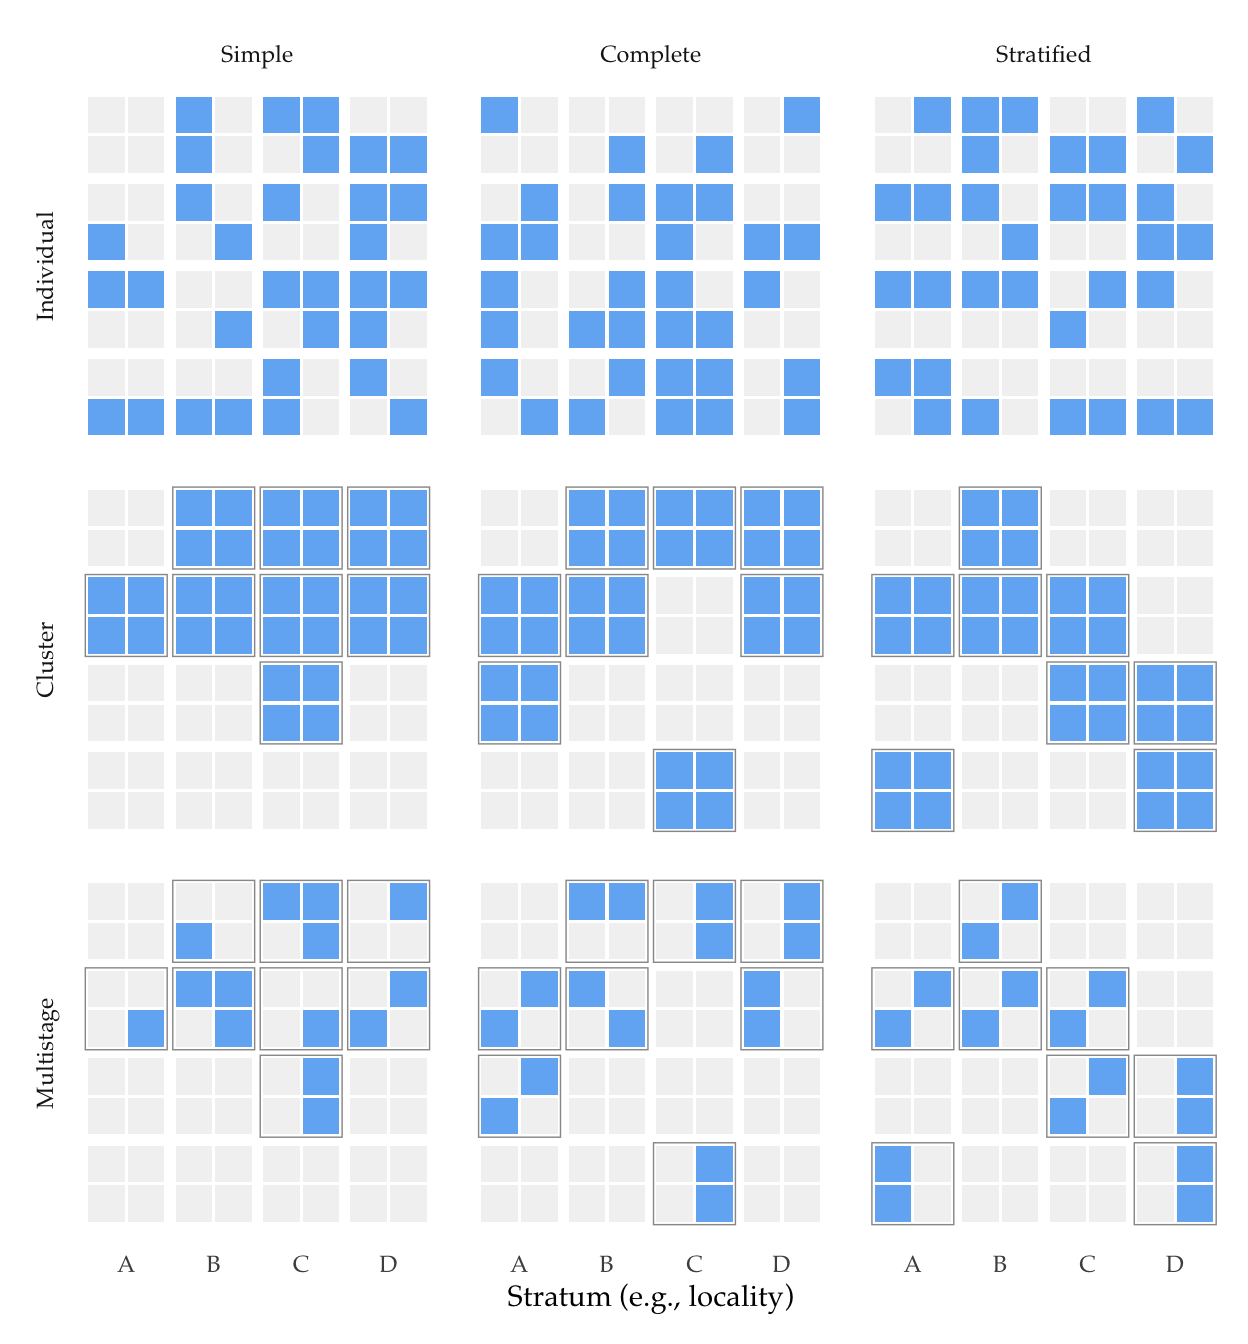
\includegraphics[width=1\linewidth]{01_Random_Sampling_files/figure-latex/unnamed-chunk-4-1}

\hypertarget{diagnosis}{%
\paragraph{Diagnosis}\label{diagnosis}}

Two main diagnosands for the simple random sampling design are bias and
rmse. We want to know if we get the right answer on average and we want
to know, on average, how far off from the truth we are.

\begin{Shaded}
\begin{Highlighting}[]
\NormalTok{diagnosands <-}\StringTok{ }\KeywordTok{declare_diagnosands}\NormalTok{(}
  \DataTypeTok{bias =} \KeywordTok{mean}\NormalTok{(estimate }\OperatorTok{-}\StringTok{ }\NormalTok{estimand),}
  \DataTypeTok{rmse =} \KeywordTok{sqrt}\NormalTok{(}\KeywordTok{mean}\NormalTok{((estimate }\OperatorTok{-}\StringTok{ }\NormalTok{estimand) }\OperatorTok{^}\StringTok{ }\DecValTok{2}\NormalTok{))}
\NormalTok{)}
\NormalTok{diagnosis <-}\StringTok{ }\KeywordTok{diagnose_design}\NormalTok{(design, }\DataTypeTok{diagnosands =}\NormalTok{ diagnosands) }
\end{Highlighting}
\end{Shaded}

\begin{table}

\caption{\label{tab:completerandomsampling}Complete random sampling design diagnosis}
\centering
\begin{tabular}[t]{ll}
\toprule
Bias & RMSE\\
\midrule
0.00 & 0.11\\
(0.01) & (0.00)\\
\bottomrule
\end{tabular}
\end{table}

The diagnosis in table @ref(tab:completerandomsampling) indicates that
under complete random sampling, the sample mean estimator of the
population mean is unbiased and that the root mean squared error is
manageable at 0.11.

\hypertarget{exercises}{%
\paragraph{Exercises}\label{exercises}}

\begin{enumerate}
\def\labelenumi{\arabic{enumi}.}
\tightlist
\item
  Can you modify the design to define the estimand as the mean of the
  latent variable \texttt{Y\_star}? What happens if you diagnose this
  design?
\item
  Can you modify the design to allow for the possibility of measurement
  error?
\item
  Can you modify the design to allow for the possibility of sampling
  error?
\end{enumerate}

\hypertarget{clustered-random-sampling}{%
\subsubsection{Clustered random
sampling}\label{clustered-random-sampling}}

Researchers often cannot randomly sample at the individual level because
it may, among other reasons, be too costly or logistically impractical.
Instead, they may choose to randomly sample households, political
precincts, or any group of individuals in order to draw inferences about
the population. This strategy may be cheaper and simpler but may also
introduce risks of less precise estimates.

Let's modify our first design to sample at the household level, rather
than at the individual individual level. We'll also add an additional
estimator that clusters standard errors at the level of sampling, the
household to compare to the estimator that ignores clustering. We'll
also add a new diagnosand, coverage, which will indicate whether the
confidence intervals we construct (which depend on the flavor of
standard errors we estimate) indeed include the true value of the
inquiry 95\% of the time.

\begin{Shaded}
\begin{Highlighting}[]
\NormalTok{design <-}
\StringTok{  }\KeywordTok{declare_population}\NormalTok{(}\DataTypeTok{data =}\NormalTok{ portola) }\OperatorTok{+}
\StringTok{  }\KeywordTok{declare_measurement}\NormalTok{(}\DataTypeTok{Y =} \KeywordTok{as.numeric}\NormalTok{(}\KeywordTok{cut}\NormalTok{(Ystar, }\DecValTok{7}\NormalTok{))) }\OperatorTok{+}
\StringTok{  }\KeywordTok{declare_estimand}\NormalTok{(}\DataTypeTok{Y_bar =} \KeywordTok{mean}\NormalTok{(Y)) }\OperatorTok{+}
\StringTok{  }\KeywordTok{declare_sampling}\NormalTok{(}\DataTypeTok{clusters =}\NormalTok{ households, }\DataTypeTok{n =} \DecValTok{50}\NormalTok{) }\OperatorTok{+}
\StringTok{  }\KeywordTok{declare_estimator}\NormalTok{(Y }\OperatorTok{~}\StringTok{ }\DecValTok{1}\NormalTok{,}
                    \DataTypeTok{model =}\NormalTok{ lm_robust,}
                    \DataTypeTok{estimand =} \StringTok{"Y_bar"}\NormalTok{,}
                    \DataTypeTok{label =} \StringTok{"Standard errors not clustered"}\NormalTok{) }\OperatorTok{+}
\StringTok{  }\KeywordTok{declare_estimator}\NormalTok{(Y }\OperatorTok{~}\StringTok{ }\DecValTok{1}\NormalTok{,}
                    \DataTypeTok{clusters =}\NormalTok{ households,}
                    \DataTypeTok{model =}\NormalTok{ lm_robust,}
                    \DataTypeTok{estimand =} \StringTok{"Y_bar"}\NormalTok{,}
                    \DataTypeTok{label =} \StringTok{"Standard errors clustered"}\NormalTok{)}

\NormalTok{diagnosands <-}\StringTok{ }\KeywordTok{declare_diagnosands}\NormalTok{(}
  \DataTypeTok{bias =} \KeywordTok{mean}\NormalTok{(estimate }\OperatorTok{-}\StringTok{ }\NormalTok{estimand),}
  \DataTypeTok{rmse =} \KeywordTok{sqrt}\NormalTok{(}\KeywordTok{mean}\NormalTok{((estimate }\OperatorTok{-}\StringTok{ }\NormalTok{estimand) }\OperatorTok{^}\StringTok{ }\DecValTok{2}\NormalTok{)),}
  \DataTypeTok{coverage =} \KeywordTok{mean}\NormalTok{(estimand }\OperatorTok{<=}\StringTok{ }\NormalTok{conf.high }\OperatorTok{&}\StringTok{ }\NormalTok{estimand }\OperatorTok{>=}\StringTok{ }\NormalTok{conf.low)}
\NormalTok{)}
\NormalTok{diagnosis <-}\StringTok{ }\KeywordTok{diagnose_design}\NormalTok{(design, }\DataTypeTok{diagnosands =}\NormalTok{ diagnosands) }
\end{Highlighting}
\end{Shaded}

\begin{table}

\caption{\label{tab:clusterrandomsampling}Cluster random sampling design diagnosis}
\centering
\begin{tabular}[t]{llll}
\toprule
Estimator Label & Bias & RMSE & Coverage\\
\midrule
Standard errors clustered & -0.01 & 0.16 & 0.96\\
 & (0.01) & (0.01) & (0.01)\\
Standard errors not clustered & -0.01 & 0.16 & 0.84\\
 & (0.01) & (0.01) & (0.02)\\
\bottomrule
\end{tabular}
\end{table}

The diagnosis shows the affect of clustering on the quality of our
estimates. While the design remains unbiased for the population mean,
the RMSE has gone up. We still interview (on average) 100 people in each
sample, but since under the clustered design, we interview all adults in
the household, the sampling distribution of the estimates has higher
variance. The diagnosis also highlights the importance of matching your
answer strategy to your data strategy. The sampling was clustered by
household. The answer strategy that fails to account for clustering
yields confidence intervals that are too small, as evidenced by the
coverage rate well below the nominal 95\%. When we estimate clustered
standard errors instead, the coverage improves.

\hypertarget{exercises-1}{%
\paragraph{Exercises}\label{exercises-1}}

\begin{enumerate}
\def\labelenumi{\arabic{enumi}.}
\tightlist
\item
  Here the clusters were defined as part of the model, but they could be
  defined as part of the data strategy. Can you modify the design and
  generate sampling clusters by putting neighboring households into the
  same cluster. Your data will have a household identifier
  \texttt{households} so you could try making a single cluster out of
  each pair (for instance households \texttt{001} and \texttt{002}). How
  does sampling using pairs households together affect your estimated
  rmse?
\end{enumerate}

\end{document}
